\documentclass{beamer}

\usepackage{times}
\usepackage[T1]{fontenc}
\usepackage{listings}
\usepackage{hyperref}
\usepackage{biblatex}
\addbibresource{presentation.bib}

\title
{Network Traffic Visualization}

\subtitle
{448.060 Advanced Computer Networks, VU}

\author
{Michael Hraschan, Thomas Unterluggauer}

\date
{WS 2011/2012}

\AtBeginSubsection[]
{
  \begin{frame}<beamer>{Outline}
    \tableofcontents[currentsection,currentsubsection]
  \end{frame}
}

\begin{document}

\lstset{language=XML,tabsize=2,basicstyle=\footnotesize,breaklines=true}

\begin{frame}
	\titlepage
\end{frame}

\begin{frame}{Table of contents}
	\tableofcontents
\end{frame}

\section{Introduction}

\section{Existing Frameworks}

\section{Implemented System}

\section{Problems}

\subsection{First Design}

\begin{frame}{The Design}
 \begin{figure}
 \centering
 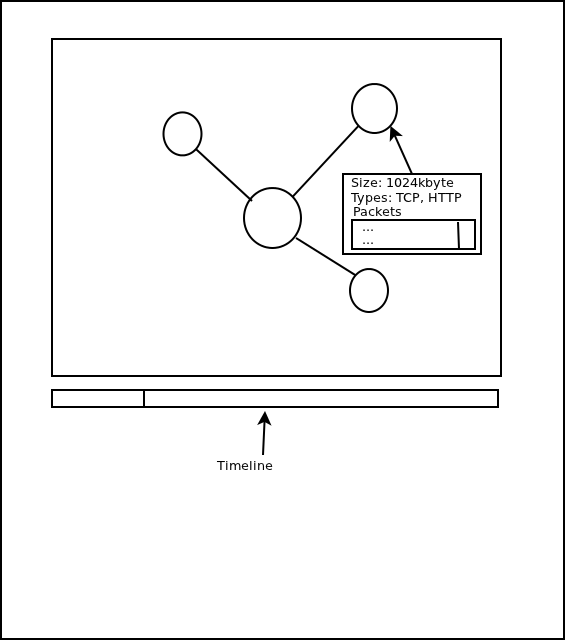
\includegraphics[width=0.9\textwidth]{./img/draft1.png}
 % draft1.png: 565x640 pixel, 72dpi, 19.93x22.58 cm, bb=0 0 565 640
 \caption{First design of the system.}
 \label{fig:draft1}
\end{figure}
\end{frame}

\begin{frame}{Ideas}
 \begin{enumerate}
  \item Everything should work smooth
  \item Show packet transfers
  \item Reload packets on demand
  \item Make it responsive
  \item Show everything in a timeline
 \end{enumerate}
\end{frame}

\subsection{Problems The 1st}

\begin{frame}
 \begin{enumerate}
  \item Web != Client application
  \item Javascript...
  \begin{enumerate}
   \item Single threaded
   \item When something ``is done'', user cannot interact
   \item Packet transfer (AJAX) pauses everything...
  \end{enumerate}
  \item So we couldnt simulate something AND be responsive

 \end{enumerate}

\end{frame}

\subsection{Second Design}

\begin{frame}{(Reduced) Ideas}
 \begin{enumerate}
  \item Let the user set a point in timeline and show the state at that time
  \item No ``fancy'' simulation stuff
  \item The rest should remain the same
 \end{enumerate}

\end{frame}


\begin{frame}{And more problems...}
 \begin{enumerate}
  \item Packets... so many packets
  \item Even a short tcpdump generates a few thousand packets
  \item Transfer every packet from server to client?
  \item Reduced information which is sent to client
 \end{enumerate}
\end{frame}

\section{Demo}

\begin{frame}{The result}
\begin{enumerate}
 \item \url{http://tcpdumpnetworkvisualizer.appspot.com}
 \item Or just a video...
\end{enumerate}
\end{frame}


\begin{frame}
  Thanks for your attention!
\end{frame}


\section{Referenzen}

\begin{frame}{References}
\printbibliography
\end{frame}


\end{document}
